%\documentclass{Physics_H_Notes}
%\begin{document}
    \section{课后习题:热力学}
    %本章习题基本等于阅读理解加背公式,知识点实在太多,不重要的公式各位考前过一下,我就不放习题了
    \begin{example}[Pressure ---\refleaftext{solution7.1}]
        In state-of-the-art vacuum systems, pressures as low as $10^{-9}\rm{Pa}$ are being attained. 
        Calculate the number of molecules in a $1.00\rm{m^{3}}$ vessel at this pressure if the temperature is 27°C
    \end{example}
    \begin{example}[Ideal gas ---\refleaftext{solution7.2}]
        In fact, the root-mean-square 
        speed of molecules in air (mostly $\rm{N_2}$) is comparable to 
        the speed of sound in air (or in an ideal gas).
        (a) Using the equation of state of an ideal gas, calculate the bulk 
        modulus (at temperature $T$), which is defined as:
        \begin{equation*}
            B = \frac{volume \ stress}{volume \ strain} = -\frac{\Delta F/A}{\Delta V/V} = -\frac{\Delta P}{\Delta V/V}
        \end{equation*}

        (b) Recall that the speed of sound in a fluid $v=\sqrt{B/\rho}$ depends on
        the elastic and inertial properties of the fluid, where $B$ is the bulk
        modulus and $\rho$ is the density of air. Express the speed of sound 
        waves in terms of molecular mass $m$, temperature $T$, as well as 
        the Boltzmann's constant $k_{_B}$.

        (c) In fact, the speed of sound has an additional factor of $\sqrt{\gamma}$ ,
        where $\gamma$ is the adiabatic index ($\gamma = 7/5 = 1.400$ for diatomic molecules 
        at room temperature). Compute the result in (b) at room temperature (The molar
        mass of air is $29 \rm{g/mol}$). 
    \end{example}
    \begin{example}[The van der Waals gas ---\refleaftext{solution7.3}]
        The van der Waals equation of state is as follows:
        \begin{equation*}
            (p+\frac{a}{V^{2}})(V-b)=nRT
        \end{equation*}
        (a) Calculate the isothermal compressibility of the van der Waals gas in terms of $(V,T)$ and
        determine the high-temperature limit. How does this result compare to that for an ideal gas?
        
        Hint: The isothermal compressibility $\kappa_T$ is defined through $\kappa_{T}=-\dfrac{1}{V}\left(\dfrac{\partial V}{\partial p}\right)_{T}$

        (b) The van der Waals equation possesses a so-called critical point, where
        \begin{equation*}
            \left(\frac{\partial p}{\partial V}\right)_{T} = \left(\frac{\partial^{2} p}{\partial V^{2}}\right)_{T} = 0
        \end{equation*}
        Determine the critical pressure $p_c$, the critical volume $V_c$ and the critical temperature $T_c$. What
        is the behavior of $\kappa_T$ at the critical point?

        (c) Use the expressions for $V_c$, $p_c$, and $T_c$ in the van der Waals equation of state and show that it
        assumes a simple form independent of $a$ and $b$ when $T$,$V$, and $p$ are measured in terms of $T_c$,
        $V_c$, $p_c$, $i.e.$, when expressing the van der Waals equation in terms of $T/T_c$ , $V/V_c$ , $p/p_c$
    \end{example}
    \begin{example}[Heat and Work ---\refleaftext{solution7.4}]
        An ideal diatomic gas, in a cylinder with a movable piston, undergoes the rectangular cyclic process shown
        . Assume that the temperature is always such
        that rotational degrees of freedom are active, but vibrational modes are “frozen out.” Also assume that the only
        type of work done on the gas is quasistatic compression-expansion work. 
        \begin{center}
            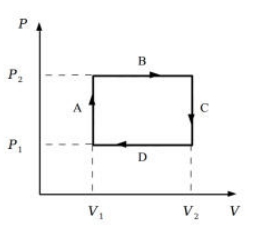
\includegraphics[height=5cm,width=5cm]{Chapter7_pV1.png}
        \end{center}
        (a) For each of the four steps A through D, compute the work done on the gas, the heat added to
        the gas, and the change in the internal energy of the gas.
        Express all answers in terms of $P_1$, $P_2$, $V_1$, and $V_2$. \\
        (b) Compute the net work done on the gas, the net
        heat added to the gas, and the net change in the internal
        energy of the gas during the entire cycle. Are the results
        as you expected? Explain briefly.
    \end{example}
    \begin{example}[Carnot Cycle ---\refleaftext{solution7.5}]
        For a van der Waals gas, its equation of state implies a phase transition between
        liquid and gas below a critical temperature $T_c$: In the $P-V$ phase
        diagram, the isothermal line for a given temperature $T_{_0} < T_{c}$ is not monotonically
        decreasing with respect toV, but a constant function of $V$ in some region (see the
        figure). This region corresponds to a phase transition from liquid to gas state (with a
        volume change from $V_{L}^{mol}$ to $V_{G}^{mol}$), and the mole latent heat is $L$ for the transition.
        Suppose we use 1 mole of this van der Waals gas/liquid mixture as the medium for
        a Carnot cycle operating between the high temperature $T_{_0}$ and the low temperature
        $T_{_0}-\Delta T$ — which are connected by two adiabatic processes $D\rightarrow A$ and $B\rightarrow C$.
        The pressure in the flat region changes from $P_{_0}$ to $P_{_0}-\Delta P$ when the temperature
        changes from $T_{_0}$ to $T_{_0}-\Delta T$.
        \begin{center}
            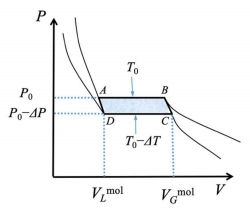
\includegraphics[height=5cm,width=6cm]{Chapter7_pV2.png}
        \end{center}

        (a) Specify the heat transfer and work done in each process of $A\rightarrow B$, $B\rightarrow C$,
        $C\rightarrow D$, and $D\rightarrow A$ in such a Carnot cycle. Here, we assume that the volume
        change in $B\rightarrow C$ and $D\rightarrow A$ is negligible.

        (b) Calculate the total work done to the environment for this Carnot cycle and express
        its efficiency $\epsilon$ from $\epsilon = W/Q_H$. where $W$ and $Q_H$ is the total work output in
        the cycle and the heat input at the high temperature, respectively

        (c) For a Carnot engine with efficiency $\epsilon = 1-\dfrac{T_C}{T_H}$, verify the Clapeyron equation:
        \begin{equation*}
            \frac{\dif{P}}{\dif{T}}=\frac{L}{T(V_{G}^{mol}-V_{L}^{mol})}
        \end{equation*}    
        for the liquid/gas mixture.
    \end{example}
    \begin{example}[Entropy ---\refleaftext{solution7.6}]
        Consider the Carnot cycle operating with a hot and cold heat baths whose temperatures are $T_h$ and
        $T_c$ ($T_h > T_c$), respectively. Working substance means the gas in the engine, and we consider a gas in
        general for the working substance.

        (a) Suppose the amount of heat exchange during the isothermal process with the hot (cold) heat bath is
        $Q_h$ ($Q_c$), and determine the entropy change $\Delta S_h$ and $\Delta S_c$ of the working substance in the respective
        process. Then, specify $\Delta S_h$ and $\Delta S_c$ are positive or negative. Here, take the positive sign of $Q_h$
        and $Q_c$ for the heat input from the heat bath to the working substance.

        (b) Now we use an ideal gas as the working substance and consider a free expansion process. Suppose the
        initial temperature of the gas is $T_i$ and the volume of the gas increases from $V_i$ to $V_f$. Determine the
        heat input $Q_{fe}$ and the entropy change $\Delta S_{fe}$ of the working substance through the free expansion
        process.

        (c) By replacing a quasi-static isothermal expansion process in the Carnot cycle by a free expansion
        process, it seems that it is possible to construct a cycle with a single heat bath. Does this fact
        violate the second law of thermodynamics? Answer by yes or no, then explain your answer using
        the case of the Carnot cycle.
    \end{example}
%\end{document}